\documentclass[11pt]{article}
\usepackage{../cs70, latexsym,epsf,amsmath,amsfonts,graphicx,url}

\lecture{6}
\def\title{Note \the\lecturenumber}

\newcounter{thm}
\addtocounter{thm}{\the\lecturenumber}

\newtheorem{theorem}{Theorem}[thm]
\newtheorem{algorithm}{Algorithm}[thm]
\newtheorem{lemma}{Lemma}[thm]
\newtheorem{fact}{Fact}[thm]
\newtheorem{definition}{Definition}[thm]
\newtheorem{conjecture}{Conjecture}[thm]
\newtheorem{counterexample}{Counterexample}[thm]
\newtheorem{corollary}{Corollary}[thm]
\newtheorem{observation}{Observation}[thm]

%%% Alistair's Macros
\makeatletter
\def\eqalign#1{\,\vcenter{\openup\jot\m@th
  \ialign{\strut\hfil${##}$&${{}##}$\hfil
      \crcr#1\crcr}}\,}
\def\eqalignno#1{\displ@y \tabskip\@centering
  \halign to\displaywidth{\hfil${##}$\tabskip\z@skip
    &${{}##}$\hfil\tabskip\@centering
    &\llap{$##$}\tabskip\z@skip\crcr
    #1\crcr}}
\makeatother
%%% End Alistair's Macros

\renewcommand{\pmod}[1]{~(\text{mod}~#1)}
\newcommand{\tmod}{\text{mod}}

\begin{document}
\maketitle

\section{Modular Arithmetic}

Suppose you go to bed at 23:00 o'clock and want to get $8$ hours of sleep. What time should you set your alarm for? Clearly, the answer is not ($23 + 8 = $) 31:00 o'clock, but rather ($31 - 24 = $) 7:00 o'clock. This is because in the 24-hour clock system the numbers ``wrap around'' back to 0:00 once we hit 24:00, so the naive answer 31:00 means the same thing as the correct answer 7:00, namely, $7$ hours after midnight.

The clock system is an example of a very useful type of arithmetic known as {\em modular arithmetic}, in which we perform all arithmetic operations relative to a fixed number $n$ called the {\em modulus}. In the $24$-hour clock system the modulus is $n = 24$, and we can write the example above as
\begin{align*}
    31 \pmod{24} ~=~ 7 
\end{align*}
which is read ``$31$ {\em modulo} $24$ is equal to $7$.'' Here the function ``$(\text{mod}~24)$'' is another name for remainder when divided by $24$. So $31 \pmod{24}$ is equal to $7$ because $31 = 1 \cdot 24 + 7$ and $0 \le 7 \le 23$.

There are many other ways we use modular arithmetic in everyday life. As another example, consider the $7$ days in a week. Suppose instead of calling them $\{$Monday, Tuesday, $\dots$, Sunday$\}$, we label them with $\{0,1,\dots,6\}$. Then we can describe the $7$-day system with arithmetic modulo $n = 7$. For instance, the sentence ``$3$ days after Sunday is Wednesday'' can be translated into the statement
\begin{align*}
    6 + 3 \pmod{7} ~=~ 2
\end{align*}
and this holds because $6+3 = 9$ and when we divide $9$ by $7$ we get a remainder of $2$. You can also see this by imagining the numbers wrapped around a circle where $7$ is identified with $0$ (see Figure~\ref{Fig:ModCircle}), so adding or subtracting numbers correspond to walking around the circle forward or backward.

\vspace{4pt}
\begin{figure}[h!]
  \centering
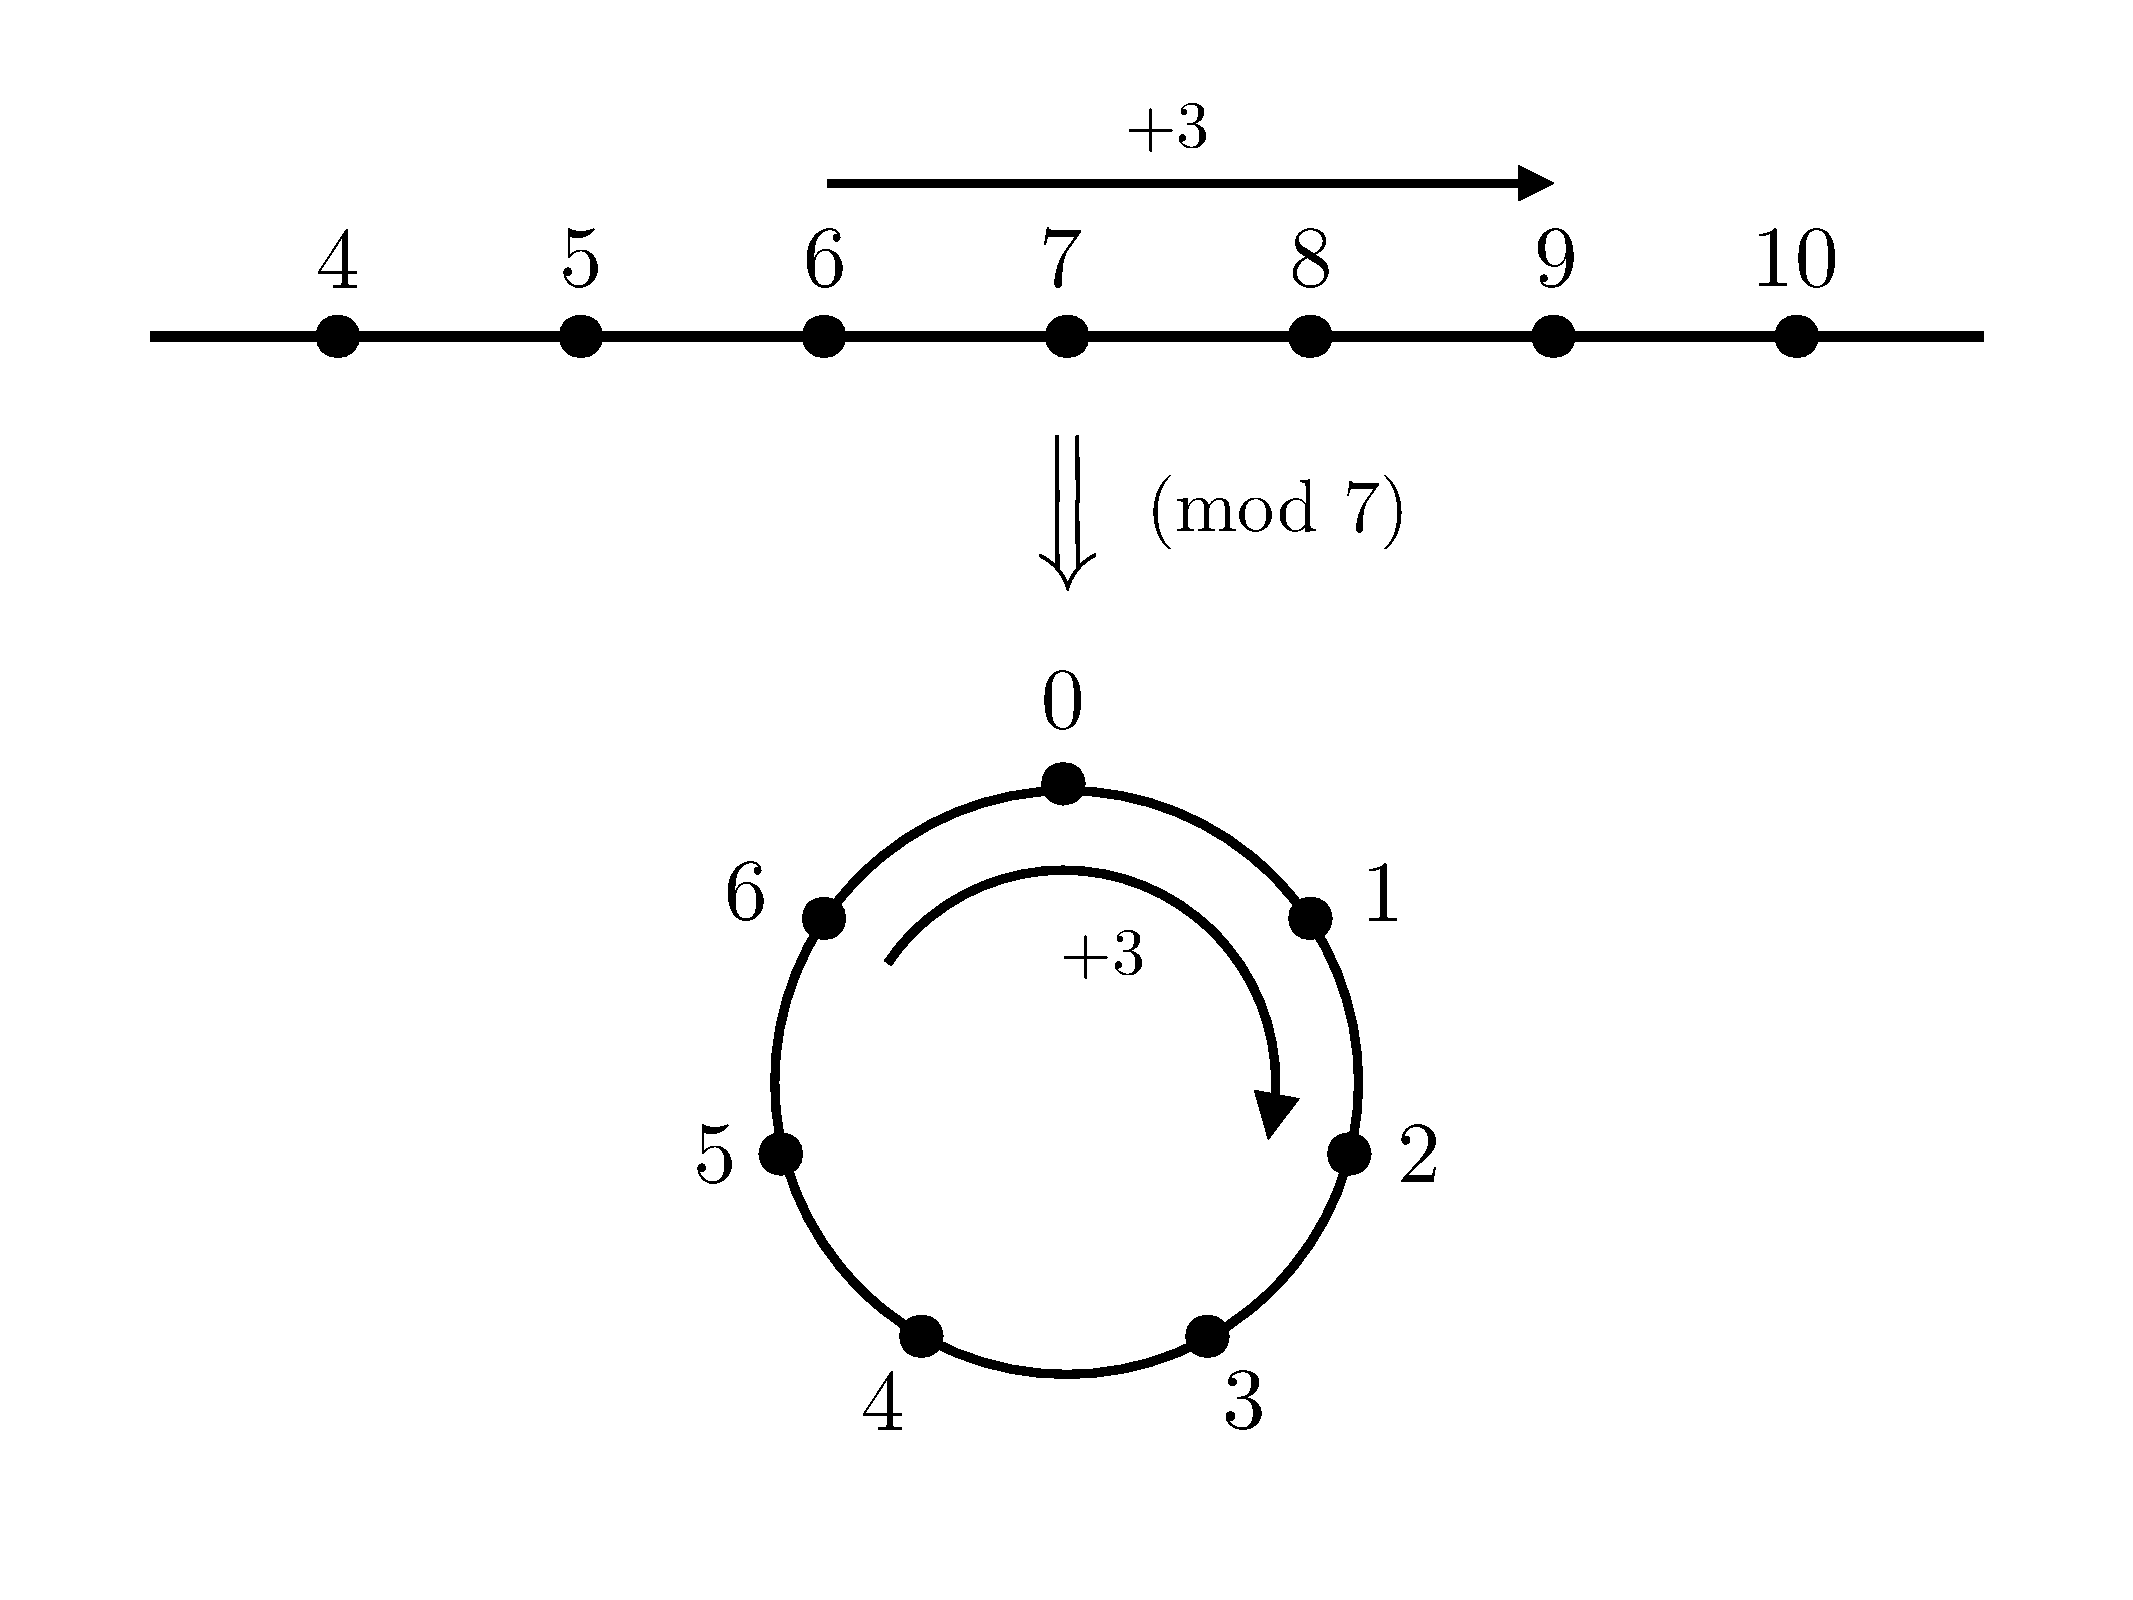
\includegraphics[width=.35\textwidth]{ModCircle}
\label{Fig:ModCircle}
\caption{Addition by $3$ on the integers (top) and modulo $7$ (bottom).}
\end{figure}
\vspace{4pt}

Convince yourself that you can do the same with the $30$ days in a month, $12$ months in a year, etc.

So far these are simple examples from everyday life. But modular arithmetic is a very useful tool that lies at the heart of many powerful results in computer science, such as error-correcting codes and cryptography, including public-key cryptosystem such as RSA. To understand these results, let us first familiarize ourselves with modular arithmetic and explore its properties.



\subsection{Addition, Subtraction, Multiplication}
\label{Sec:ModAdd}

One of the most important properties of numbers modulo $n$ is that the familiar arithmetic operations give robust results. The best way to illustrate this is by example. Suppose we wish to compute $42 + 35 \pmod{24}$. Here are two different ways of doing so. One way is to first compute the addition, then reduce $(\text{mod}~24)$:
$$42 + 35 \pmod{24} ~=~ 77  \pmod{24} ~=~ 77 - 72 ~=~ 5.$$
The second way is to first apply $(\text{mod}~24)$ to each term, add the results, and finally apply $(\text{mod}~24)$ again:
$$42 + 35 \pmod{24} ~=~ [42 \pmod{24}] + [35 \pmod{24}] \pmod{24} ~=~ 18 + 11 \pmod{24} ~=~ 29 \pmod{24} ~=~ 5.$$
You see that we still get the same answer as before.
This is no coincidence. We can perform any sequence of arithmetic operations $(\text{mod}~24)$ and the result is robust --- 
it remains unchanged whether we reduce $(\text{mod}~24)$ only once at the end of all operations, or we reduce each intermediate result $(\text{mod}~24)$, or even if we reduce some intermediate results $(\text{mod}~24)$ at whim as long as we reduce the final 
answer $(\text{mod}~24)$. Why is this the case? To see this we must view numbers modulo $n$ in a completely different way. 

For two integers $a$ and $b$, let us define $a$ to be {\em congruent} to $b$ modulo $n$, written
$$a ~\equiv_n~ b$$
if and only if $a \pmod{n} = b \pmod{n}$, i.e., $a$ and $b$ give the same remainder when divided by $n$. 
In the above scenario, this captures the property that $a$ and $b$ would result in the same answer when used in the arithmetic operations. Here is another way of
saying the same thing:
$$a \equiv_n b ~~ \Leftrightarrow ~~ n \:|\: (a-b)$$
(recall that $p \:|\: q$ means $p$ divides $q$, i.e., $q/p$ is an integer). 
Equivalently, we can write $a = b + k \cdot n$ for some integer $k$. Make sure you understand and can 
show that these conditions are all saying the same thing. 

So when $n = 24$, all these numbers are congruent to each other:
$$\dots ~\equiv_{24}~ -48 ~\equiv_{24}~ -24 ~\equiv_{24}~ 0 ~\equiv_{24}~ 24 ~\equiv_{24}~ 48 ~\equiv_{24}~ \dots$$
Similarly,
$$\dots ~\equiv_{24}~ -47 ~\equiv_{24}~ -23 ~\equiv_{24}~ 1 ~\equiv_{24}~ 25 ~\equiv_{24}~ 49 ~\equiv_{24}~ \cdots$$
and so on. Indeed, you can see that there are $24$ such sets where the numbers within each set are all congruent to each other.

The reason that arithmetic modulo $n$ is robust is that all the arithmetic operations --- plus, minus, times --- respect these sets. This is proved in
the following theorem:

\begin{theorem}
\label{Thm:Mod1}
For all $n \ge 1$ and $a,b,c,d \in \Z$, the following are true:
\begin{enumerate}
  \item If $a \,\equiv_n\, b$ and $c \,\equiv_n\, d$, then $a+c \,\equiv_n\, b+d$
  \item If $a \,\equiv_n\, b$ and $c \,\equiv_n\, d$, then $a\cdot c \,\equiv_n\, b\cdot d$
\end{enumerate}
\end {theorem}

\begin{proof}
We prove part (1). The proof of (2) is left as an exercise.

Since $a \,\equiv_n\, b$, there exists $k \in \Z$ such that $a = b + k \cdot n$. Similarly, since $c\,\equiv_n\, d$, there exists $\ell \in \Z$ such that $c = d + \ell \cdot n$. Then we can write
$$a+c = (b+d) \,+\, (k+\ell) \cdot n$$
which means $(a+c) - (b+d)$ is divisible by $n$. This shows that $a+c \,\equiv_n\, b+d$. 
\end{proof}

{\bf Remark:} In our notation so far, $(\text{mod}~n)$ is a function that maps an integer $a$ to an element in the set $\{0,1, \ldots, n-1\}$ by computing the remainder when dividing $a$ by $n$. The notation $\equiv_n$ says that two integers give the same remainder when divided by $n$. These two concepts are related, but quite different from each other. Once we get used to the two concepts, it is customary to blur the distinction between them and use the notation $(\text{mod}~n)$ interchangeably: to denote the remainder, but also to denote equivalence as in
$$a ~\equiv~ b \pmod{n}$$
to denote $a \,\equiv_n\, b$.



%%%%%%%%%%%%%%%%%%%%
\section{Division and Multiplicative Inverses}


In Section~\ref{Sec:ModAdd} we discussed addition, subtraction, and multiplication in the setting of modular arithmetic. Curiously, we left out division. The reason is that division is a bit more tricky in this setting, and thus warrants its own discussion. To begin, let's recall how division is done over the rational numbers $\Q$. Here, if we want to divide $x\in\Q$ by $y\in \Q$, we can equivalently multiply by $y^{-1}$, where if $y=a/b$, then $y^{-1}=b/a$. The term $y^{-1}$ has a special name --- it is a \emph{multiplicative inverse} of $y$, i.e. a number such that $y\cdot y^{-1}=1$. This suggests the following approach for dividing number $x$ by $y$ in modular arithmetic: Simply multiply $x$ by $y^{-1}$.

But what is the multiplicative inverse of $y$ modulo $n$? Is it unique as in the case of working over the rationals? Even more troubling --- is it clear the inverse even \emph{exists}? Remarkably, both scenarios are possible in modular arithmetic: Sometimes the inverse doesn't exist, and sometimes it does. When it \emph{does} exist, however, it turns out to be unique. Let's explore these ideas further.

Consider the case of $x=8$. Does $x$ have a multiplicative inverse modulo $n=15$? Yes! Note that $2x\,\equiv\,16\,\equiv\,1\pmod{15}$. Thus, $2$ is a multiplicative inverse of $x$ modulo $15$.

\sanity{Consider now $x=12$ and $n=15$. Does $x$ have a multiplicative inverse modulo $m$? (Hint: Since we are working modulo $15$, there are only $15$ possible choices for the inverse. Try plugging in $a=0,1,2,\ldots$ into $a x \pmod n$ and seeing if you get the answer $1$. Do you see a pattern forming?)}

So sometimes the inverse exists, and sometimes it does not. Is there a way to distinguish between the two cases? Yes --- it turns out that $x$ has a multiplicative inverse modulo~$n$ if and only if the greatest common divisor of $n$ and $x$ is 1. Here, the {\em greatest common divisor} of two natural numbers $x$ and $y$,
denoted $\gcd(x,y)$, is the
largest natural number that divides them both.
For example, $\gcd(30, 24) = 6$.
If $\gcd(x,y)=1$, it means that $x$ and $y$ share
no common factors (except~1); in this case we call $x$ and $y$ {\it relatively prime}.

\sanity{What is $\gcd(21, 49)$? How about $\gcd(12,13)$?}

We can show that the multiplicative inverse exists precisely when the number $x$ is relatively prime to the modulus $n$. The proof is left as an exercise.

\begin{theorem}\label{thm:inverse}
Let $n,x$ be positive integers. Then $x$ has a multiplicative inverse modulo~$n$ if and only if $\gcd(n,x) = 1$. Moreover, if it exists, then the multiplicative inverse is unique.
\end{theorem}

%\begin{theorem}\label{thm:inverse}
%Let $n,x$ be positive integers such that $\gcd(n,x)=1$.
%Then $x$ has a multiplicative inverse modulo~$n$, and it is unique
%(modulo~$n$).
%\end{theorem}
%\begin{proof}%[Proof of Theorem~\ref{thm:inverse}]
%Consider the sequence of $n$ numbers $0,\,x,\,2x,\,\ldots,\,(n-1)x$.
%We claim that these are all distinct modulo~$m$.  Since there
%are only $m$ distinct values modulo~$n$, it must then be the case
%that $a x \,\equiv\, 1\pmod n$ for exactly one~$a$ (modulo~$m$).  This~$a$
%is the unique multiplicative inverse.
%
%To prove the above claim, suppose for sake of contradiction that $ax \, \equiv \,  bx \pmod n$ for
%two distinct values $a,b$ in the range $0 \le b < a \le n-1$.
%Then we would have $(a-b)x \,\equiv\, 0 \pmod n$, or equivalently,
%$(a-b)x\,=\,kn$ for some integer~$k$.
%
%However, $x$ and $n$ are relatively prime, so $x$ cannot
%share any factors with $n$. This implies that $a-b$ must
%be an integer multiple of $n$. This is not possible, since $a-b$ ranges
%between $1$ and $n - 1$.
%\end{proof}


%Using similar techniques, you can also prove that $\gcd(n,x)=1$ is a {\it necessary\/}
%condition for the existence of an inverse: In other words, if $x$ has a multiplicative inverse modulo $n$, then $\gcd(n,x)=1$. Finally, since Theorem~\ref{thm:inverse} says that whenever the inverse exists, it is \emph{unique}, we can denote the inverse of $x$ (assuming it exists) as $x^{-1}\pmod n$.

\subsection{Computing the Multiplicative Inverse}\label{sscn:computeinverse}

Theorem~\ref{thm:inverse} gives us a sufficient condition for determining if a multiplicative inverse of $x$ modulo $n$ \emph{exists}. But it doesn't tell us how to \emph{find} such an inverse! In this section, we discuss an efficient algorithm for computing the inverse itself whenever it exists. Interestingly, this task is closely related to computing the greatest common divisor of two numbers, and both go via variants of \emph{Euclid's algorithm}. It is worth noting that the latter is one of the oldest algorithms still in use, dating back to around 300 BC!

%Being able to compute the multiplicative inverse of a number is crucial to many applications, so ideally the algorithm used should be efficient. It turns out that we can use an extended version of Euclid's algorithm, which computes the gcd of two numbers, to compute the multiplicative inverse.

To begin, let us see how computing the multiplicative inverse of $x$ modulo $m$ is related to finding $\gcd(x,m)$. Suppose that for any pair of numbers $x,y$, we can not only compute $\gcd(x,y)$, but also a pair of integers $a,b$ satisfying
\begin{equation}\label{extEuclid}
   d \,=\, \gcd(x,y) \,=\, ax+by.
\end{equation}
(Note that this is not a modular equation, and the integers
$a,b$ can be zero or negative.)  For example, we can write
$1=\gcd(35,12)=-1\cdot 35 + 3\cdot 12$, so here $a=-1$ and $b=3$
are possible values for $a,b$.

%\sanity{
%Show that the integers $a,b$ in~\eqref{extEuclid} are not unique. (Hint: Show that if $a,b$ satisfy~\eqref{extEuclid}, then so do $a+y,b-x$.)
%}


If we can do this, then we can compute the multiplicative inverse of $x$ modulo $n$ as follows. First, compute integers $a$ and $b$
such that 
$$
   1=\gcd(n,x) = an+bx.  
$$
This implies, however, that $bx \, \equiv \, 1\pmod n$. Thus, $b$ must be the
multiplicative inverse of~$x$ modulo~$n$! Reducing $b$ modulo~$n$
hence gives us the \emph{unique} inverse we are looking for.  
\sanity{
In the example $1=\gcd(35,12)=-1\cdot 35 + 3\cdot 12$, what is the unique multiplicative inverse $12^{-1}$ of $12$? Verify your answer by explicitly checking that indeed $12\cdot 12^{-1}\,\equiv\,1 \pmod{35}$.
}

% show that the pair of integers is not unique. Hint: show that if (a,b) is a pair then (a+x,b+y) is a pair. 

We conclude that we have reduced the problem of computing inverses to the problem of finding integers $a,b$ satisfying Equation~(\ref{extEuclid}). Remarkably, Euclid's algorithm for computing greatest common divisor \emph{also} allows us to find the integers $a$ and $b$ described above, which we shall see now. %So, computing the multiplicative inverse of $x$ modulo $m$ is as simple as running Euclid's gcd algorithm on input $x$ and $m$!


\subsubsection{Euclid's Algorithm}

We begin by describing the ``basic'' version of Euclid's algorithm, which only computes the gcd, and not the integers $a$ and $b$ as described in Equation~(\ref{extEuclid}). In the next section, we describe the \emph{extended} version of Euclid's algorithm, which completes both tasks, as promised.

To begin, suppose we wish to compute the gcd of two numbers $x$ and $y$. An easy ``base case'' is when either $x$ or $y$ is 0; for example, if $x=0$, then $\gcd(x,y)=y$, since $0$ is divisible by everything. In a nutshell, Euclid's algorithm works by reducing the general case of computing $\gcd(x,y)$ down to this base case. To accomplish this, we need the following theorem that allows us to reduce the size of the integers that we are working with, thereby getting us closer to the base case.

\begin{theorem}\label{thm:samediv}
Let $x \geq y$ and let $q, r$ be natural numbers such $x = yq + r$ and $r < y$.
Then $\gcd(x,y) = \gcd(y,r)$.
\end{theorem}

\begin{proof}
We give a direct proof. Note that the claim will follow if we can show that any common divisor $d$ of $x$ and $y$ is also a common divisor of $r$ and $y$, and vice versa. To show the forward direction, suppose $d \mid x$ and $d \mid y$. This means $z = x / d$ and $w = y / d$ are integers. Then we see that
$$r \,=\, x - yq \,=\, zd - wdq \,=\, (z - wq)d$$
implying $d\mid r$, as desired. The converse direction follows similarly.
\end{proof}

\exercise{Show the converse direction of the proof of Theorem~\ref{thm:samediv}, i.e., show that $d\mid y$ and $d\mid r$ imply $d\mid x$.}

Given this theorem, let's see how to compute $\gcd(16,10)$. We begin by writing
\[
	16= 10\times 1 + 6.
\]
Here $x = 16$, $y = 10$, $q = 1$, and $r = 6$. By Theorem~\ref{thm:samediv}, we know that $\gcd(16,10)=\gcd(10,6)$. Therefore, we can simplify the problem by now focusing on $\gcd(10,6)$, and writing
\[
	10= 6 \times 1 + 4.
\]
As before, Theorem~\ref{thm:samediv} says $\gcd(10,6)=\gcd(6,4)$. You can probably see a pattern forming now. We apply the same idea on $\gcd(6,4)$, and so forth, obtaining the sequence of equations:
\begin{eqnarray*}
	6 &=& 4 \times 1 + 2\\
	4 &=& 2\times 2 + 0\\
	2 &=& 0\times 0 + 2.
\end{eqnarray*}
Note that the last line is precisely the base case we discussed at the start of this section --- we are looking for $\gcd(2,0)$, which is trivially $2$. We conclude that $\gcd(16,10)=2$, as desired. %Or if you %wish you can stop a step earlier and say that the gcd is the last non-zero
%remainder: i.e. you can stop at the step $6 = 4 \times 1 + 2$, since at the next step the remainder is $0$.

\sanity{Apply the algorithm sketched above to compute $\gcd(24, 12)$.}

Now that you've had a chance to get your hands dirty by trying out the algorithm, let's describe it formally using recursion as follows.

{\obeylines \tt
~~// precondition: Assumes $x \geq y \geq 0$ and $x>0$.
~~// postcondition: Outputs $\gcd(x,y)$.
~~{\bf algorithm} $\gcd(x,y)$
~~\quad if $y = 0$ then return $x$
~~\quad else return $\gcd(y, \: x \; (\text{mod}~y))$}
~~\par\smallskip\noindent

You should run through a second quick example to convince yourself that this formal description really does capture the algorithm we sketched previously.
\sanity{Compute $\gcd(32,10)$ using the formal algorithm above.}

\subsubsection{Extended Euclid's Algorithm}
We finally give an extended version of Euclid's algorithm which computes $\gcd(x,y)$, along with integers $a$ and $b$ satisfying $\gcd(x,y) = ax+by$, allowing us to finally compute multiplicative inverses. The algorithm is as follows.

%Now since this problem is a generalization of the basic gcd,
%it is perhaps not too surprising that we can solve it
%with a fairly straightforward extension of Euclid's algorithm.
%\subsubsection*{Examples}
%Let's first see how we would compute such numbers for $x = 6$ and
%$y = 4$. We'll need the equations from our example above, copied here for reference:
%
%$16= 10\times 1 + 6$\\
%$10= 6 \times 1 + 4$\\
%$6 = 4 \times 1 + 2$\\
%$4 = 2\times 2 + 0$\\
%
%From the last two equations it follows that $\gcd(6,4) = 2$. But now the second last
%equation gives us the numbers $a, b$, since we just rearrange that equation to
%say $2 = 6\times 1 - 4 \times 1$. So $a = 1$ and $b = -1$.
%
%What if we started with $x = 10$ and $y = 6$? Now we would write the last three equations to
%determine that $\gcd(10, 6) =2$. But how do we find $a, b$? Start as above and write
%$2 = 6\times 1 - 4 \times 1$. But we want $10$ and $6$ on the right hand side, not $6$ and $4$.
%But notice that the third from the last equation allows us to write $4$ as a linear combination
%of $6$ and $10$ and so we can just back substitute: we rewrite that equation as
%$4 = 10\times 1 - 6 \times 1$ and substitute to get: \\
%$2 = 6\times 1 - 4 \times 1 = 6\times 1 - (10\times 1 - 6 \times 1) = 6 \times 2 - 10 \times 1$.
%
%If we started with $x = 16$ and $y = 10$ we would back substitute again using the
%first equation rewritten as $6 = 16 - 10$ to get:\\
%$2 = 6 \times 2 - 10 \times 1 = (16 - 10) \times 2 - 10 = 16 \times 2 - 10\times 3$.
%So $a = 2$ and $b = -3$.
%
%\iffalse
% To find the
%numbers $a$ and $b$ described above, we can rewrite the equation as:
%$$
%2 = 2 - 0\times 0
%$$
%Hence $a = 1$ and $b = 0$. What about $\gcd(4,2)$? Now we need
%the last two equations. We first write $2 = 2 - 0\times 0$, as above.
%The second to last equation can be rewritten as $0 = 4 - 2\times 2$,
%and now we can substitute this expression for 0:
%$$
%2 = 2 - 0\times 0 = 2 - 0\times(4 - 2\times 2) = 0\times 4 + 1\times 2.
%$$
%We have now found $a$ and $b$ for $\gcd(4,2)$: $a=0$ and $b=1$.
%
%We computed $a$ and $b$ by back substituting in the equations used to compute
%the gcd. We can continue this method for longer examples, such as computing $\gcd(16,10)$.
%We first write \\
%$2 = 0\times 4 + 1\times 2$ as computed above.\\
%Now substitute $2 = 6 - 4\times 1$:\\
%$2 = 0\times 4 + 1 \times (6 - 4\times 1)$\\ or
%$2 = 1\times 6 - 1\times 4$\\
%Now substitute $4 = 10 - 6\times 1$:\\
%$2 = 1\times 6 - 1\times (10-6\times 1)$\\ or
%$2 = -10 + 2 \times 6$\\
%Now substitute $6 = 16 - 10\times 1$:\\
%$2 = -10 + 2\times (16 - 10\times 1)$\\ or
%$2 = 2 \times 16 - 3 \times 10$\\
%So $a = 2$ and $b = -3$.
%\fi
%
%\iffalse
%$2 = 6 - 4\times 1$\\
%Now substitute $4 = 10 - 6\times 1$:\\
%$2 = 6 - (10-6\times 1)\times 1$\\ or
%$2 = -10 + 6 \times 2$\\
%Now substitute $6 = 16 - 10\times 1$:\\
%$2 = -10 + (16 - 10\times 1)\times 2$\\ or
%$2 = 16 \times 2 - 10 \times 3$\\
%So $a = 2$ and $b = -3$.
%\fi
%\subsubsection*{Algorithm}
%The following recursive
%algorithm {\it extended-gcd\/} implements the idea used in the examples above.
%It takes as input a pair of natural
%numbers $x\ge y$ as in Euclid's algorithm, and returns a triple
%of integers $(d,a,b)$ such that $d=\gcd(x,y)$ and $d=ax+by$:
\par\smallskip
{\obeylines \tt
~~//precondition:\;\:Assumes $x\geq y\geq 0$ and $x>0$.
~~//postcondition:\;\:Outputs $(d,a,b)$ where $d=\gcd(x,y)$ and $a,b \in \Z$ with $d=ax+by$.
~~{\bf algorithm} $\text{extended-gcd}(x,y)$
~~\quad if $y = 0$ then return $(x, 1, 0)$
~~\quad else
~~\quad\quad let $(d, a, b) := \text{extended-gcd}(y, \: x \; (\text{mod} y))$
~~\quad\quad return $(d,\,b,\,a - \lfloor x/y\rfloor b)$
}
\par\smallskip\noindent
Here the {\em floor} $\lfloor z \rfloor$ is the largest integer $c$ such that $c \le z$.

Note that the extended gcd algorithm has the same form as the basic gcd algorithm we saw earlier; the only difference is that we now also carry around the values $a,b$. Let's make sure you believe this algorithm does what we claim via an example.

\sanity{Run $\text{extended-gcd}(x,y)$ on inputs $x=16$ and $y=10$. Check that the resulting values of $a$ and $b$ indeed satisfy the postcondition that $d=ax+by$.}

Finally, to understand \emph{why} this algorithm works, let us prove its correctness!

\begin{theorem}
	If $x$ and $y$ satisfy the preconditions of extended-gcd, then the output $(d,a,b)$ of $\text{extended-gcd}(x,y)$ satisfy its postconditions.
\end{theorem}
\begin{proof}
%You'll see a full analysis of this algorithm in CS 170, including
%correctness and efficiency (the running time is $O(n^3)$) . Let us understand intuitively why the numbers
%$a$ and $b$ returned by the algorithm should give us what we are looking for. We just need
%to generalize the back substitution method we used in the example above.
We proceed by strong induction on $y$. The base case is $y=0$, in which case the algorithm returns $(d,a,b)=(x,1,0)$. This is correct since $x=\gcd(x,0)$ and $x=1\cdot x+ 0\cdot y$, as desired. Assume now the claim is true for all $0<y\leq k$. We prove the claim for $y=k+1$. Let $x$ and $y$ be the input to $\text{extended-gcd}$. Then by the induction hypothesis, the first line in the {\tt else} clause returns $(d,a,b)$ such that $d=\gcd(y, \: x \; \pmod y)$ and $d=ay+ b \, (x \: \pmod y)$. Thus, our job is to check that the last line of the algorithm returns values satisfying the postcondition, i.e., that $d=\gcd(x,y)$ and that $d=bx+(a - \lfloor x/y\rfloor b)y$. The first of these is correct by Theorem~\ref{thm:samediv}. To see the second,  note that we can write~$x\:\pmod y = x - \lfloor x/y\rfloor y$ (check this!), so
%The algorithm reduces finding $\gcd(x,y)$ to finding $\gcd(y,x\bmod y)$. Once the algorithm
%finds $\gcd(y,x\bmod y)$, it returns
%values $a$ and $b$ such that:
%\begin{equation}\label{extEuclid2}
%   d=ay+b(x\bmod y).
%\end{equation}
%
%Now we need to update these values of $a$ and $b$, say to $A$ and $B$, such that
%\begin{equation}\label{extEuclid3}
%   d = Ax + By.
%\end{equation}
%To figure out what $A$ and $B$ should be, we need to rearrange
%equation~(\ref{extEuclid2}), as follows: 
\[
	d = ay+b \, (x \: \pmod y)= ay + b \, (x - \lfloor x/y\rfloor y)= bx + (a - \lfloor x/y\rfloor b) y.
\] 
This concludes the proof.
\end{proof}








%%%%%%%%%%%%%%%%%%%%%%%%%%%%%%%%
\section{Practice Problems}\label{scn:problems}

\begin{enumerate}
    \item Complete the proof of Theorem~\ref{Thm:Mod1}.
    %
    \item Prove Theorem~\ref{thm:inverse}.
%    \item Prove the converse of Theorem~\ref{thm:inverse}, i.e., show that if $x$ has a multiplicative inverse modulo $n$, then $\gcd(n,x)=1$.
    %
    \item Prove that the product of any $k \ge 1$ consecutive integers is divisible by $k$.
    %
\end{enumerate}



\end{document}


